% ! TeX root = ../../main.tex
\chapter{Implementazione}
In questo capitolo vengono trattate le implementazioni e i pattern utilizzati per raggiungere i requisiti di progettazione presentati nel capitolo precedente. Sono presentate le effettive schermate ottenute partendo dai mockup mostrandone porzioni di codice particolarmente interessanti o dove sono stati applicati pattern.

\section{Integrazione totem e app BoschettoAR}
L'integrazione fra totem e l'app ha richiesto un'analisi sulla disponibilità e praticabilità di utilizzare determinate tecnologie per l'interazione fra i due dispositivi anche in un'ottica di \textit{user experience}, usabilità e scalabilità.

Per questo progetto si è optato per un'integrazione basata sul \textit{cloud computing} e più precisamente utilizzando un servizio \textit{cloud-based} per la memorizzazione in tempo reale dei dati. Viene utilizzato il prodotto Firebase Realtime di Google \cite{firebase} che offre, anche gratuitamente, scalabilità, affidabilità, facilità d'uso e sicurezza.
Scegliendo questo modo d'integrazione si apre la possibilità di aggiungere nel tempo nuove totem interattivi per l'espansione del progetto in altre sedi dell'Università di Bologna.

\`E' stato considerato l'utilizzo della tecnologia NFC per il trasferimento dei dati da APP a totem interattivo ma la mancanza dell'hardware necessario, e considerando che non tutti gli smartphone (in particolare quelli meno recenti) possiedono tale tecnologia, si è deciso di non utilizzarla.

Come ulteriore alternativa  per il caricamento dei dati da parte dell'APP si è valutato l'utilizzo di una architettura client-server e di API esposte dal web-server installato sul totem. Quest'ultima opzione sarebbe stata un buon compromesso in termini di sicurezza e velocità di trasmissione ma poco scalabile e limitando la condivisione dei dati a solo quegli utenti connessi alla rete WiFi dell'Ateneo in sede a Cesena.


\section{Organizzazione progetto}
I file del progetto sono organizzati in cartelle relative a ciascuna schermata, componente o funzionalità. L'albero delle cartelle viene presentato nel listato \ref{lst:projectDir} dove vengono espanse solo le cartelle di primo livello (model, views e dataProvider). All'interno della cartella \texttt{model} sono state inserite le classi che definiscono il modello dei dati utente (file \texttt{share\_data\_model.dart}) e i metodi/classi/interfacce di utilità (file \texttt{obj2map.dart}), in \texttt{views} sono presenti i file delle schermate raccolti in cartelle e infine in \texttt{dataProvider} sono contenuti tutti i provider di dati utilizzati dal \texttt{DataManager} (file \texttt{data\_manager.dart}) per il reperimento delle informazioni.

\begin{lstlisting}[language=C, caption={Albero della directory del progetto TotemBoschettoAR}, label={lst:projectDir}]
    TotemBoschettoAR/
        |
        +- model/
            |
            +- obj2map.dart
            +- share_data_model.dart
        +- views/
            |
            +- common/
            +- navigation_menu/
            +- home_page/
            +- stats_page/
            +- chart_page/
            +- info_page/
            +- home_page.dart
            +- stats_page.dart
            +- chart_page.dart
            +- info_page.dart
        +- dataProvider/
            |
            +- firebase_provider.dart
        +- unit_converter.dart
        +- data_manager.dart
        +- main.dart
\end{lstlisting}

\section{App Mobile}
Seguendo i mockup sono state sviluppate le diverse schermate per la condivisione dei progressi. Sono state effettuate alcune modifiche come si può notare dagli screenshot in figura \ref{fig:shareDataApp}: in sostituzione al nickname utente impostato è stata messa una breve indicazione, che si trovava precedentemente nella pagina di scansione, sul come visualizzare il QR code del totem e infine la schermata di caricamento è stata modificata sostituendo l'icona e mostrando un testo che informi l'utente del caricamento dei dati.
\begin{figure}[h!]
    \centering
    \subfloat[Pagina di condivisone progressi]{
        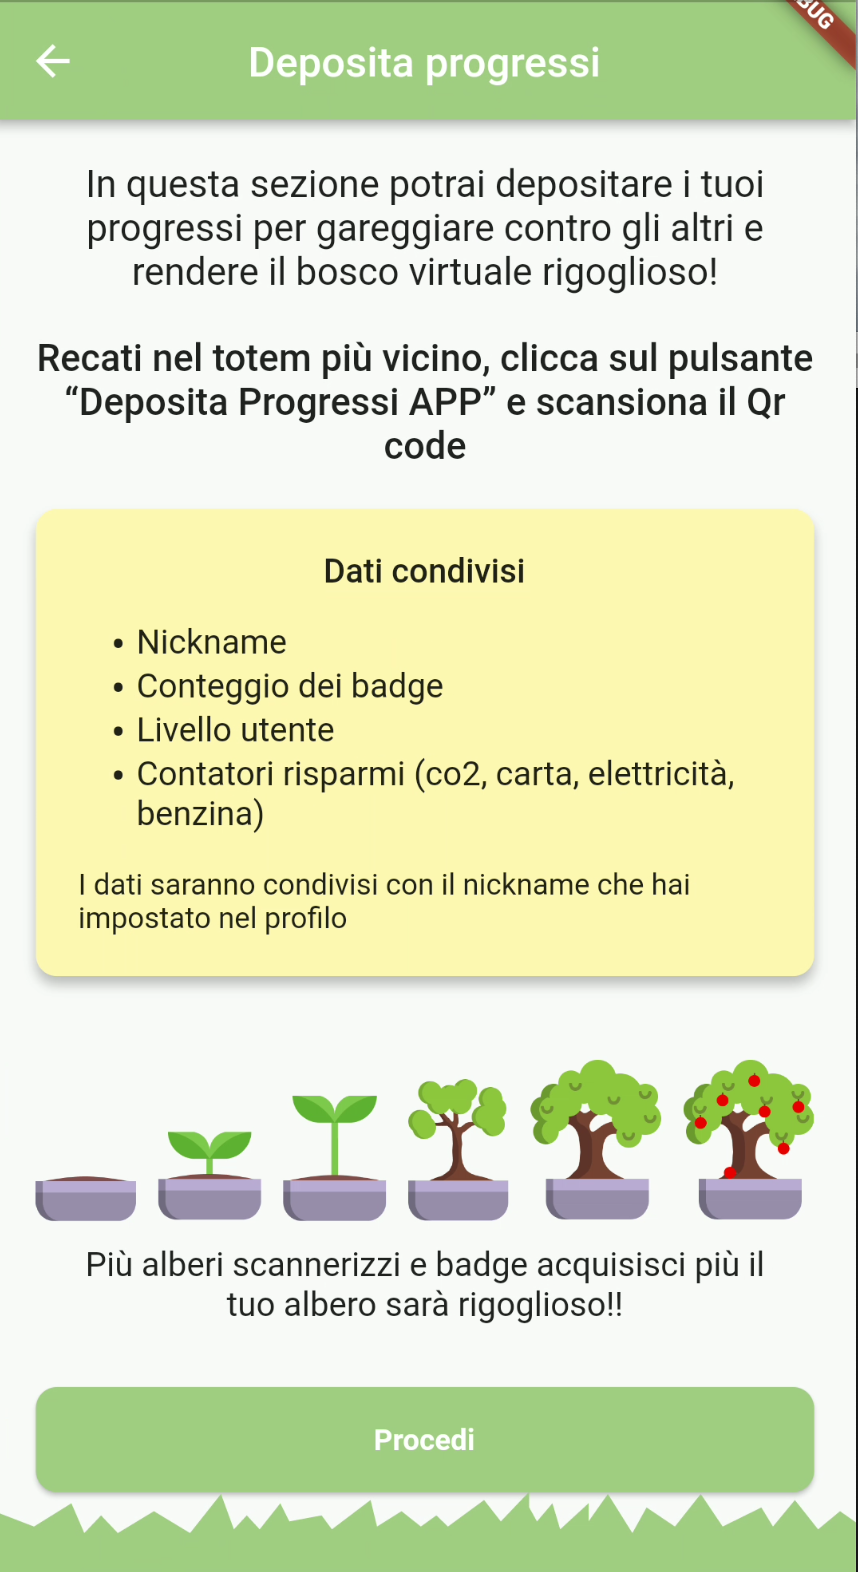
\includegraphics[width=0.3\textwidth]{img/app/uploadPage.png}
        \label{fig:sharePage}
    }
    \subfloat[Scansione QR code totem]{
        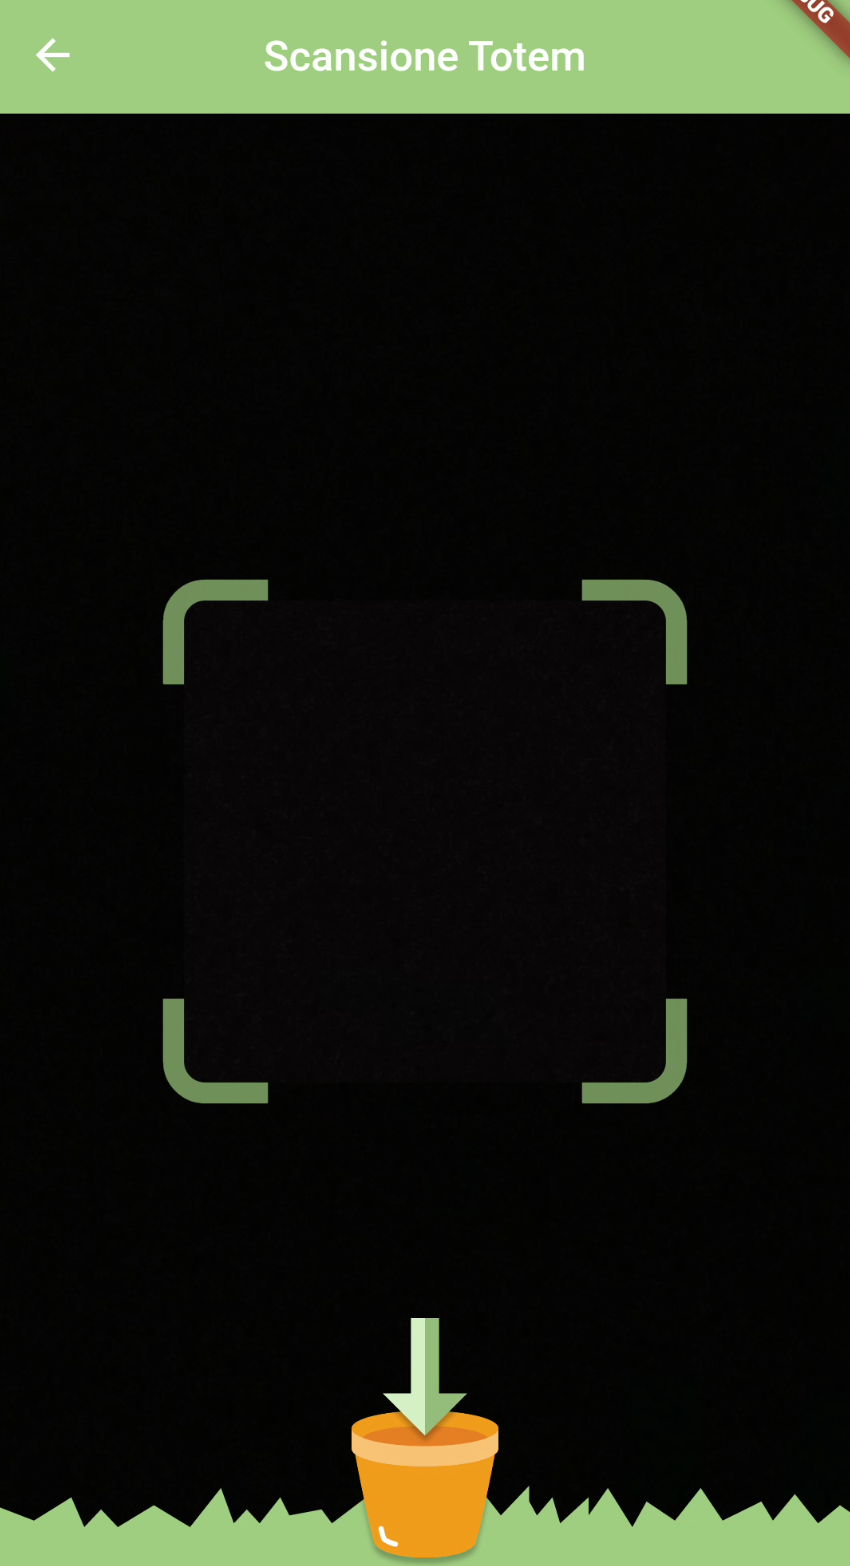
\includegraphics[width=0.3\textwidth]{img/app/uploadProgress.png}
        \label{fig:scanTotem}
    }
    \subfloat[Schermata di caricamento progressi]{
        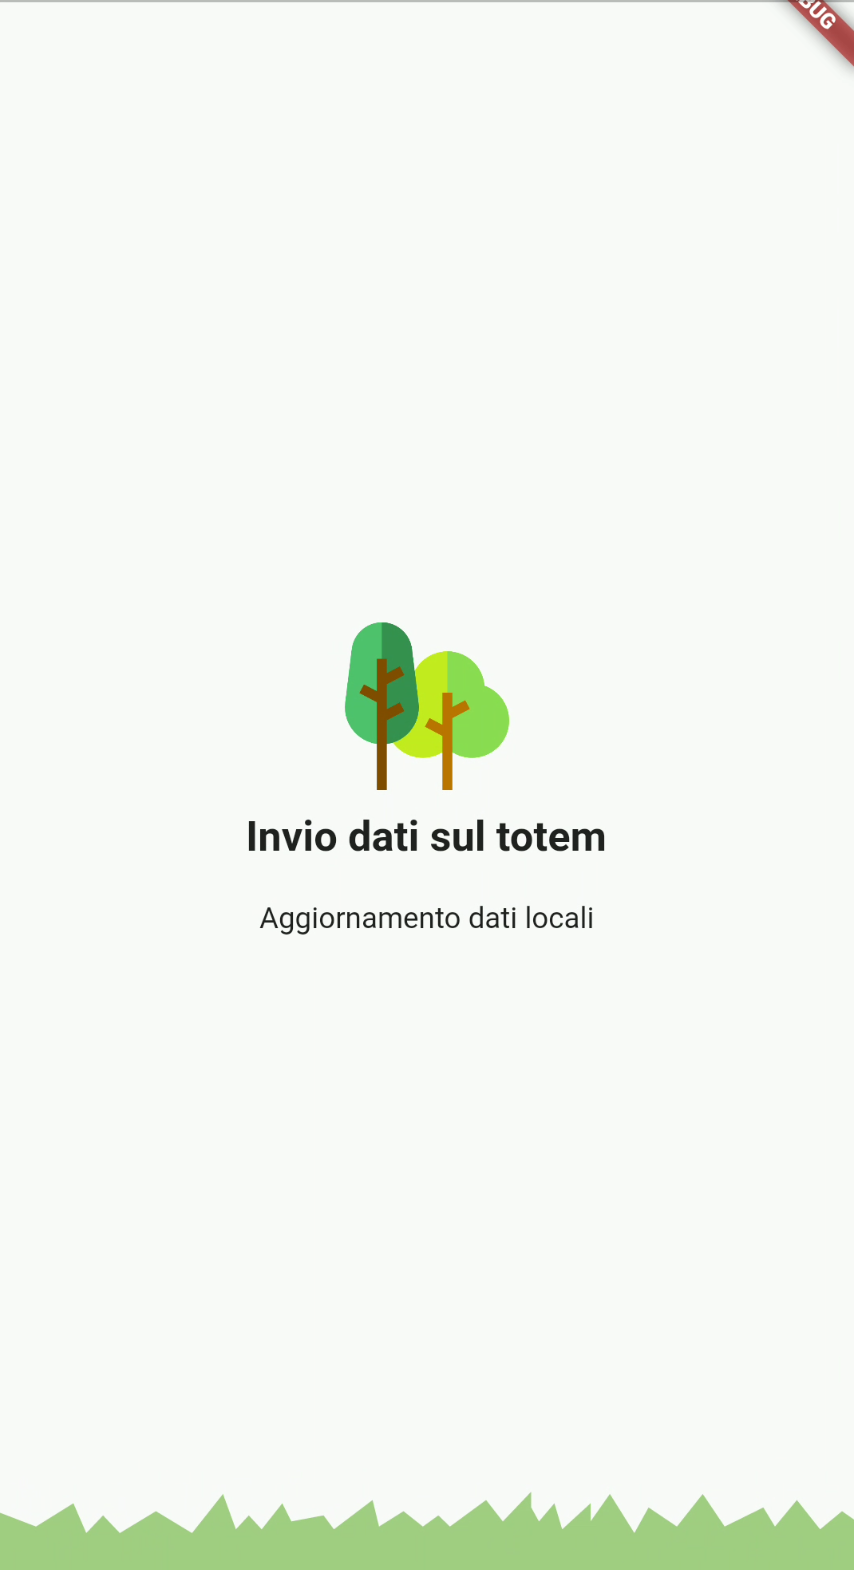
\includegraphics[width=0.3\textwidth]{img/app/uploadingPage.png}
        \label{fig:uploadinData}
    } 
    \caption{Screenshot schermate condivisione dati da app, scansione totem e caricamento}
    \label{fig:shareDataApp}
\end{figure}

\subsection{Pagina di condivisione progressi}
La schermata di caricamento dei progressi è raggiungibile dalla pagina utente oppure direttamente dalla pagina \textit{Home} in cui vi sono gli alberi collezionati. Nella barra degli strumenti (\texttt{AppBar}) di entrambe le pagine è stato aggiunto un pulsante (\texttt{IconButton})che permette di aprire la pagina di condivisione aggiungendola allo stack di schermate dell'app chiamando il metodo \textit{push} della classe \texttt{Navigator} che disciplina la navigazione fra pagine. Nel listato \ref{lst:shareIconButton} da riga 7 a riga 20 inclusa viene mostrato il codice inserito.

\begin{lstlisting}[style=FlutterStyle, caption={Codice aggiornato della barra degli strumenti dell'app: inserito pulsante per la condivisione dei progressi.}, label={lst:shareIconButton}]
    Scaffold (
      backgroundColor: Colors.white,
      appBar: AppBar(
        centerTitle: true,
        backgroundColor: mainColor, 
        title: const Text("Profilo"),
        leading: IconButton(
          onPressed: () => Navigator.push(
            context,
            MaterialPageRoute(builder: (context) {
              return const SharePorgressPage();
            }),
          ),
          icon: const Icon(
            Icons.upload,
            size: 25,
            semanticLabel: "Carica progressi",
          ),
        ),
      ),
      body: //contenuto della pagina Utente o della Home
    );
\end{lstlisting}

\subsection{Scansione QR e caricamento}
% Implementazione della schermata di scansione del qr del riutilizzo della schermata di scansione (forze pattern strategy), con schema d'interfaccia volendo 
% Implementazione della schermata con codice effettivo dell'implementazione del pattern mvi
\textcolor{red}{TODO: RIFORMULARE , IL CONCETTO è QUELLO}

La schermata della scansione del codice QR del totem prevede il riutilizzo della stesso componente utilizzato nella scansione del QR dell'albero. Infatti come si può vedere in figura ??, la schermata di scansione fa uso della classe \texttt{ScanQRView} che gestisce la fotocamera e la lettura dei codici QR. Riconosciuto un codice QR le informazioni contenute al suo interno vengono passate alla classe specifica per il totem che verifica la validità delle informazioni per poi procedere con la preparazione e caricamento dei progressi utente. Durante tutte le due fasi viene visualizzata la schermata in figura \ref{fig:uploadinData} che risulta reattiva in attesa di un esito del caricamento o della validità del codice QR.

Consiste specie di pattern strategy E in cui oltre la strategia che viene utilizzata per la validazione del codice QR scansionare si indica anche la schermata barra interfaccia utente che deve essere visualizzata dopo la scansione del codice. Ciò schermata poi possiede la sua strategia per validare ed utilizzare i dati presi dal QR.
\textcolor{red}{scegli se mettere solo future builder o tutta la classe}

 \begin{lstlisting}[style=FlutterStyle, caption={}, label={lst:strategyViewTotem}]
  Consumer<DataManager>(
    builder: (context, dataManager, child) => FutureBuilder<bool>(
      future: dataManager
          .uploadUserData(totemId)
          .timeout(const Duration(seconds: 8)),
      builder: (context, snap) {
        ConnectionState conState = snap.connectionState;
        bool uploadDone = snap.hasData ? snap.data! : false;
        if (conState == ConnectionState.waiting) {
          return const UploadingDataView();
        } else if (conState == ConnectionState.done) {
          if (uploadDone) {
            return const CompletedUploadView();
          } else {
            return const ErrorView(message: "Errore invio dati");
          }
        } else {
          return const ErrorView(message: "Errore sconosciuto");
        }
      },
    ),
  ),
\end{lstlisting}
%%%%%%%%%%%%%%%%%%%%% TOTEM %%%%%%%%%%%%%%%%%%%%%%%%%%%%%%%%
\section{Totem}
\subsection{Dati Firebase}
Una volta deciso di utilizzare il database Firebase Realtime, che è di tipo documentale, si è reso necessario convertire lo schema UML in figura \ref{fig:totemDomain} in formato JSON per avere la struttura generale dei dati che verranno memorizzati.
Per non avere troppi oggetti annidati, si è deciso di separare le informazioni del totem (listato \ref{lst:totemInfo}) dai dati utente che sono stati condivisi tramite app (listato \ref{lst:userDataTotem}).

\begin{lstlisting}[language=json, caption={Esempio di oggetto JSON contenente le informazioni sui totem}, label={lst:totemInfo}]
    "totemInfo": {
        "totemIdString": {
          "place": "locationName",
          "project": "projectName"
        },
      },
\end{lstlisting}  

\begin{lstlisting}[language=json, caption={Esempio di oggetto JSON che memorizza i dati utente per ciascun Totem}, label={lst:userDataTotem}]
      "totems": {
        "ces_remade": {
          "userNickname": {
            "badgeCount": 0,
            "co2": 0,
            "level": 0,
            "nickname": "userNickname",
            "paper": 0,
            "treesCount": 0
          }
        }
      }
\end{lstlisting}

\subsection{DataManager}
Il DataManager, come spiegato nel capitolo del design, funge sia da Repository che da Model del pattern MVI. Mantiene al suo interno i riferimenti ai diversi provider di cui fa uso, al momento solo \texttt{FirebaseProvider}, ed espone metodi che restituiscono degli \textit{State} indirizzati alla \textit{View} contenenti i dati utili alle schermate. A livello implementativo gli \textit{State} sono un oggetto della classe \texttt{Future} e vengono utilizzati come risultato ad una computazione asincrona permettendo di svolgerne altre finché non viene completata. Utilizzando \texttt{Future} come tipo di ritorno dei metodi del DataManager in combinazione con il \texttt{FutureBuilder}, si individua una forma di pattern MVI con la possibilità di adattare la View in base allo stato della computazione.

La classe \texttt{DataManager}, come si può notare in riga 1 del listato \ref{lst:dataManager}, estende \texttt{ChangeNotifier} e questo permette di aggiornare la View con i nuovi dati aggiornati.
Inoltre viene utilizzato il pattern Observer sul FirebaseProvider: il DataManager, implementando l'interfaccia \texttt{FirebaseObserver} e aggiungendosi come observer (riga 8 listato \ref{lst:dataManager}), viene notificato per qualsiasi genere di modifica dei dati nel cloud.
In cascata quindi ogni modifica sul database nel cloud fa scattare l'aggiornamento delle Views con il metodo \texttt{notifyListeners} (riga 24 listato \ref{lst:dataManager}).

\begin{lstlisting}[style=FlutterStyle, caption={Classe DataManager}, label={lst:dataManager}]
  class DataManager extends ChangeNotifier implements FirebaseObserver {
    final String _totemId = "ces_remade";
    late final FirebaseProvider _firebaseProvider;
  
    DataManager() {
      _firebaseProvider = FirebaseProvider(_totemId);
      _firebaseProvider.addObserver(this);
    }
  
    String getCurrentTotemId() {
      return _totemId;
    }
  
    Future<List<SharedData>> getData() async {
      return _firebaseProvider.getTotemData();
    }
  
    Future<List<SharedData?>> getTop10User() async {...}
  
    Future<Map<StatId, String>> getStatistics() async {...}
  
    @override
    void firebaseNotify() {
      notifyListeners(); 
    }
  }
\end{lstlisting}

\subsection{Pagina Home} 
Per la pagina principale è stata sviluppata l'idea del mockup in figura \ref{fig:forestHome} dove vengono visualizzate le chiome d'albero degli utenti che insieme compongono un bosco rigoglioso in quanto più affine all'idea di bosco virtuale. Con una visualizzazione di questo genere gli utenti hanno una maggiore percezione del senso di comunità e ciascuno può contribuire a rendere il bosco più verde e ricco di alberi. In figura \ref{fig:homepage} viene mostrata una istantanea della homepage mentre nel listato \ref{lst:homepageCode} è possibile consultare il codice che si occupa della disposizione degli alberi a riga 8 e del loro comportamento al tocco in riga 14.

Per questa pagina, come per le altre, è stata utilizzata sempre la stessa metodologia e architettura del codice per la loro creazione: con l'ausilio del \texttt{FutureBuilder} è stata sviluppata la View con la possibilità di gestire con maggiore semplicità ed astrazione l'invio degli \textit{Inten}s al Model (metodi della classe \texttt{DataManager}) e la ricezione degli \textit{State} di risposta.

\begin{figure}[h]
  \centering
  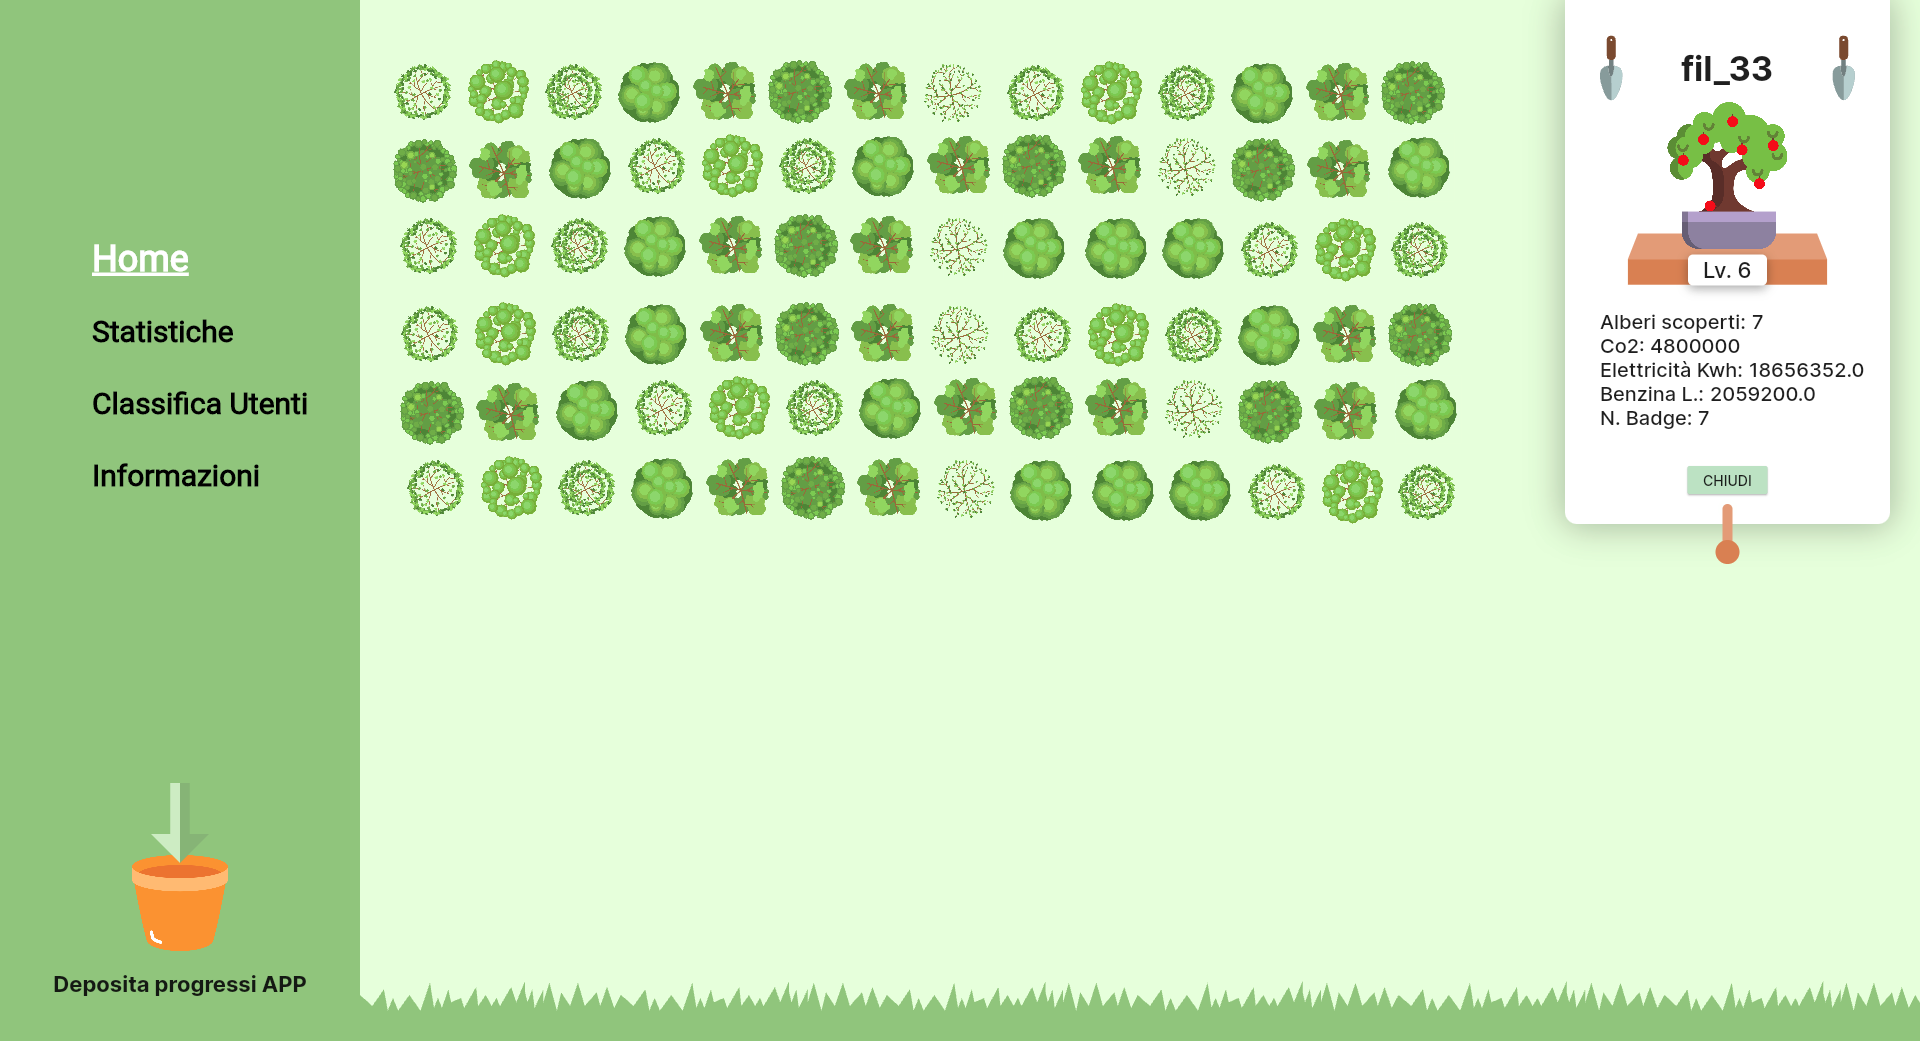
\includegraphics[width=\textwidth]{img/totem/screenshot/homepage.png}
  \caption{Screenshot della pagina Home dove viene visualizzato il bosco virtuale costruito dalla partecipazione degli utenti.}
  \label{fig:homepage}
\end{figure}

\newpage
\begin{lstlisting}[style=FlutterStyle, caption={Parte del codice per la creazione del bosco della Homepage}, label={lst:homepageCode}]
Consumer<DataManager>( // model
builder: (context, dataManager, child) =>
    FutureBuilder<List<SharedData>>(
    future: dataManager.getData(), // intent
    builder: (context, state) { // state 
      if (state.hasData) {
        // widget per la disposizione a griglia delle chiome
        return GridView.count( // view
          crossAxisCount: 20,
          mainAxisSpacing: 10,
          crossAxisSpacing: 10,
          children: (state.data ?? []).map(
            (userDataTree) {
              return GestureDetector(
                onTap: () {
                  setState(() {
                    userData = userDataTree;
                    showDetails = !showDetails;
                  });
                },
                // chioma dell'albero dell'utente
                child: ForestTree(level: userDataTree.level),
              );
            },
          ).toList(),
        );
      } else {
        return const Center(
            child: CircularProgressIndicator(
          color: Color.fromRGBO(161, 204, 130, 1),
        ));
      }
    },
  ),
),
\end{lstlisting}
%
%
\subsection{Pagina Statistiche}
\textcolor{red}{ operazioni che vengono svolte all'interno di data manager per ricavare i dati, i cerchi alla fine sono tutti colorati non sono indicatori gauge come si era pensato}
Anche questa pagina prevede l'utilizzo delle classi \texttt{Consumer<DataManager>} e \texttt{FutureBuilder<DataManager>} per rispettivamente avere accesso al DataManager e poter richiedere e ricevere i dati statistici. Inoltre per la disposizione a griglia di sei colonne e tre righe dei contatori è stato utilizzato il costruttore \texttt{GridView.count(...)}.
%TODO: PARLARE DI COME VENGONO PRESI I DATI DAL CLOUD
\subsubsection{Contatore}
Il contatore è frutto della composizione di semplici elementi grafici sovrapposti fra di loro; osservando l'immagine \ref{fig:statCont3d} partendo sinistra si ha un cerchio verde, uno bianco più piccolo, un'immagine e al di sotto una descrizione testuale. Al tocco i cerchi cambiano forma diventando quadrati, l'icona si sposta verso l'alto rimpicciolendosi lasciando al testo che viene mostrato.
\begin{figure}
  \centering
  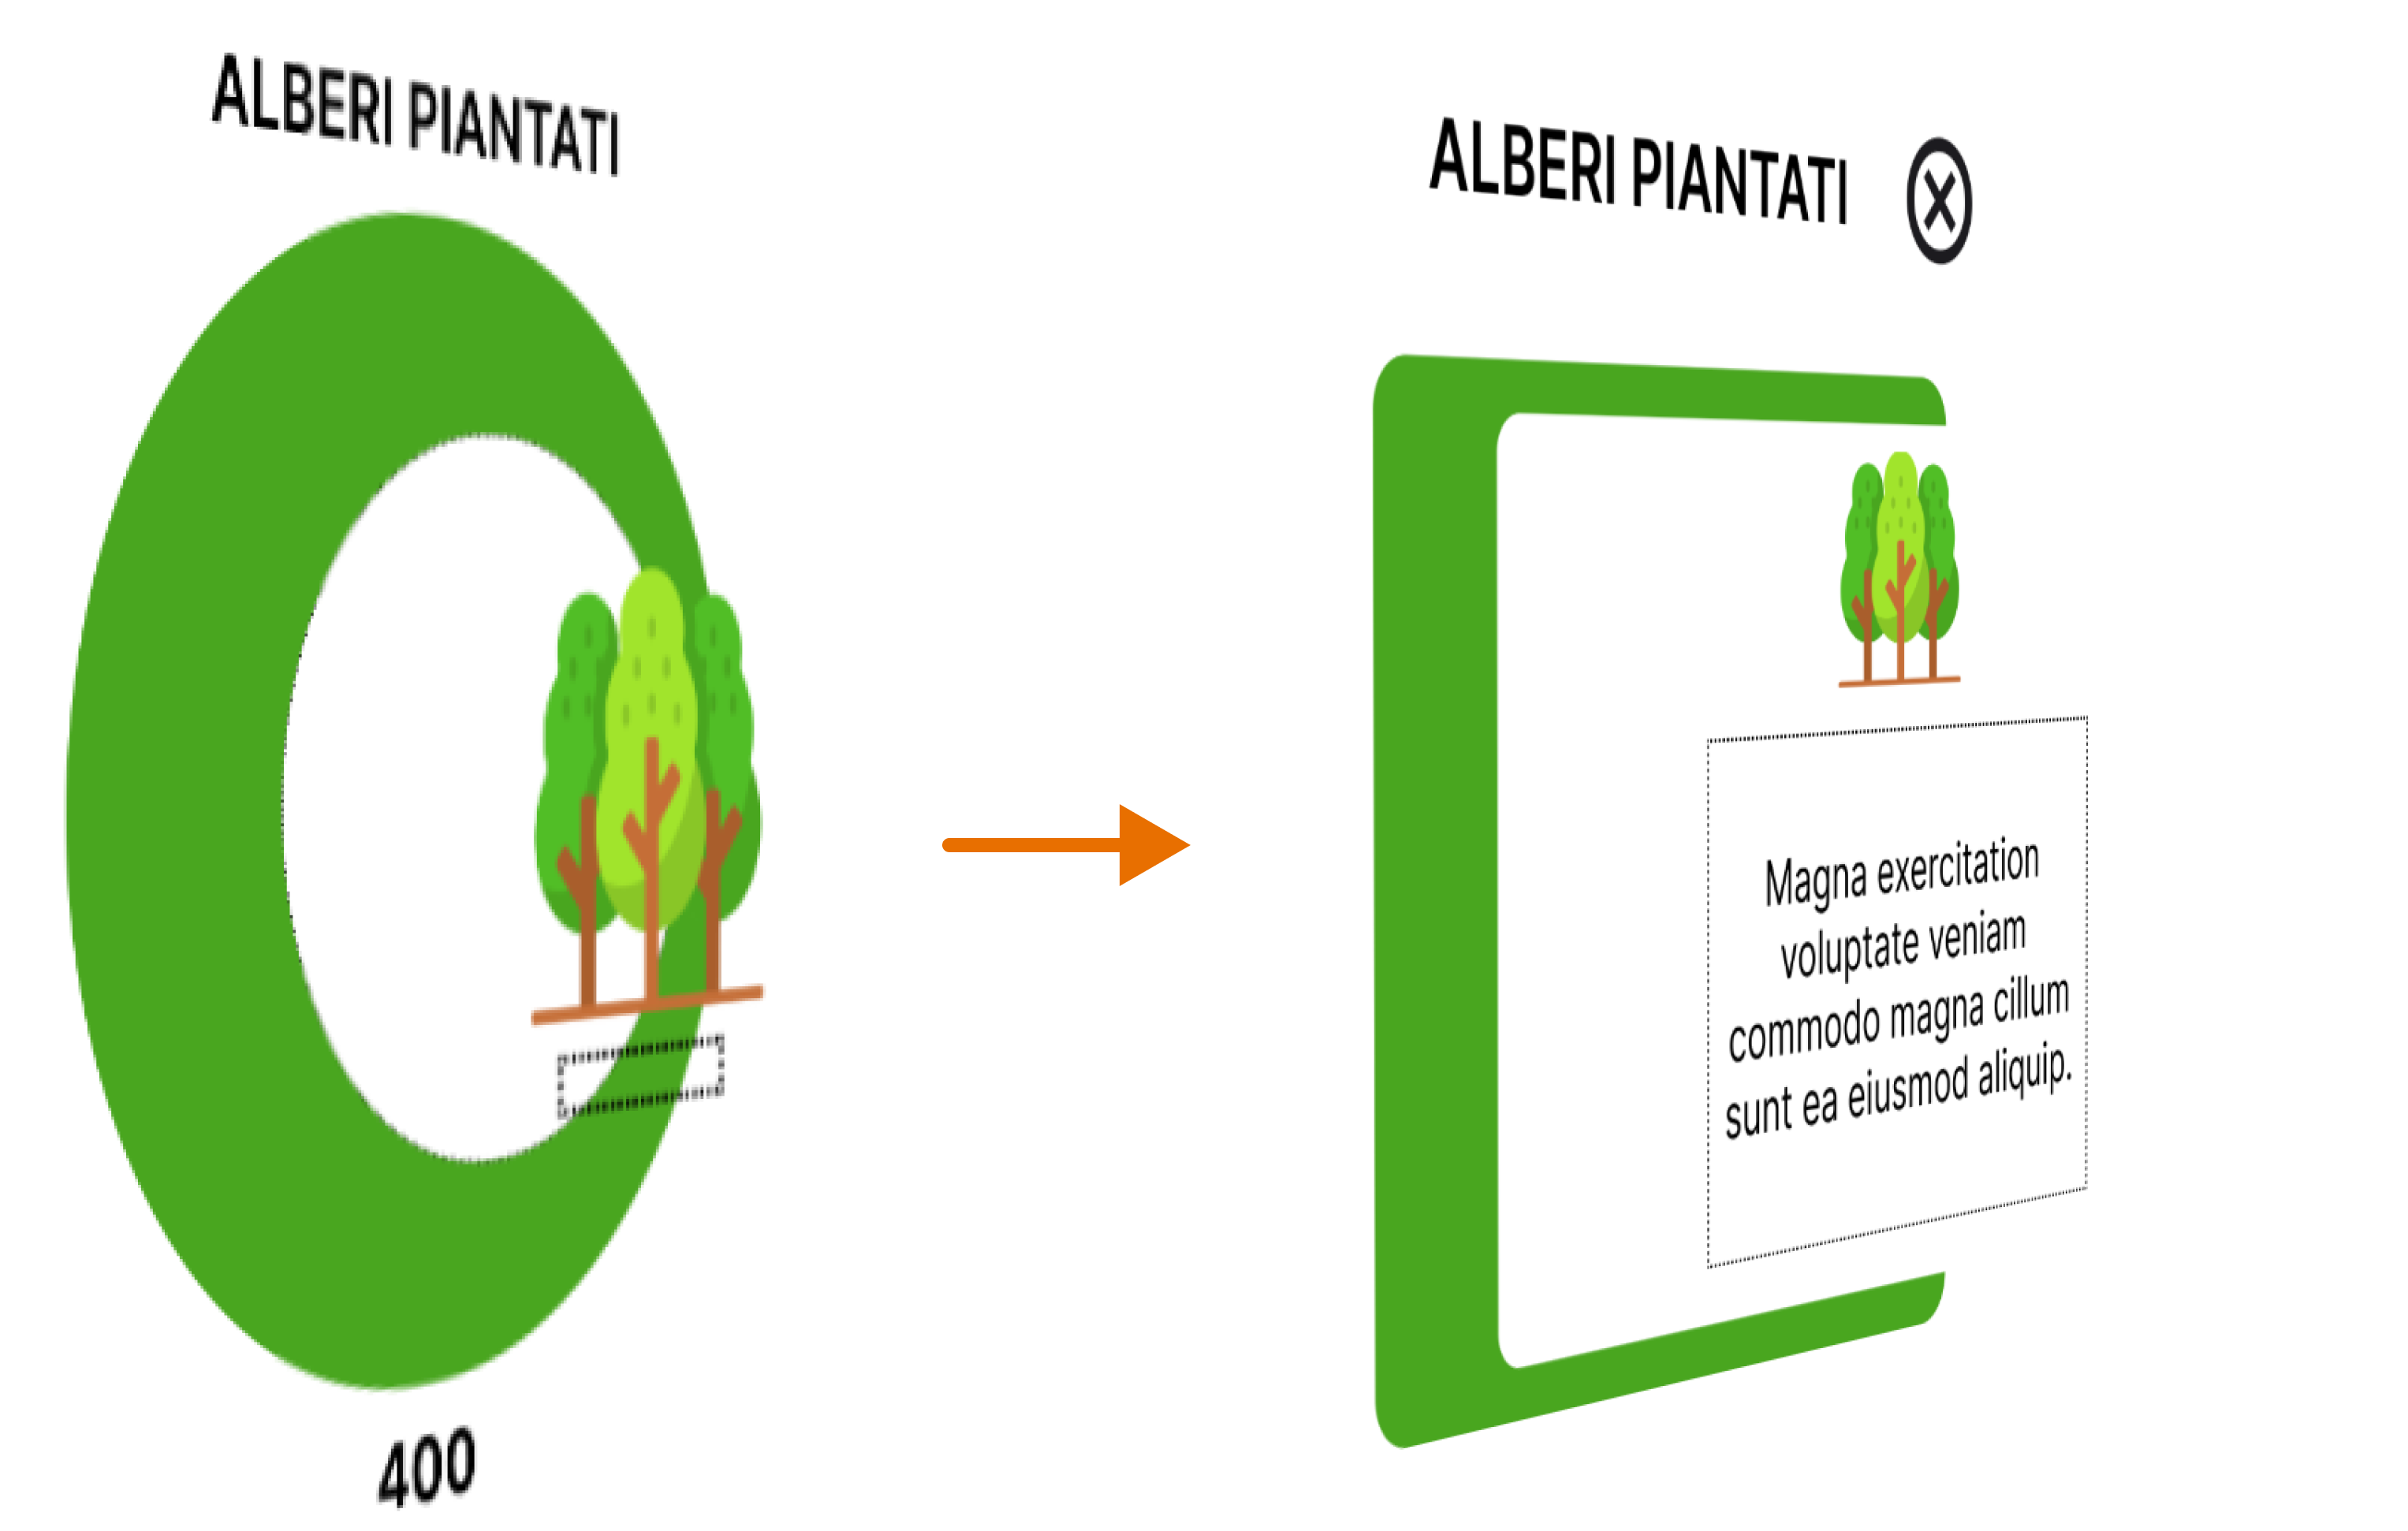
\includegraphics[width=8cm]{img/totem/statsItem3d.png}
  \caption[Contatore statistica come composizione di widget]{Contatore delle statistiche come composizione di widget: un quadrato all'interno dell'altro con sopra un'immagine e un testo (rettangolo tratteggiato).}
  \label{fig:statCont3d}
\end{figure}
%

I cerchi/quadrati vengono implementati (listato \ref{lst:roundedBox}) con la classe \texttt{RoundedBox} che restituisce un \texttt{AnimatedContainer} che è una classe che permette di animare il \textit{container}\footnote{widget di convenienza che combina widget comuni di pittura, posizionamento e dimensionamento} restituito ogni volta che viene modificata una sua caratteristica; in questo caso ad ogni tocco viene modificato il raggio del bordo (\textit{borderRadius}).

\begin{lstlisting}[style=FlutterStyle, caption={Classe RoundedBox per usata nella creazione del contatore delle statistiche}, label={lst:roundedBox}]
class RoundedBox extends StatefulWidget {
  final Color color;
  final double size;
  final double radius;

  const RoundedBox(
      {super.key,
      required this.color,
      required this.size,
      required this.radius});

  @override
  State<StatefulWidget> createState() => RoundedBoxState();
}

class RoundedBoxState extends State<RoundedBox> {
  @override
  Widget build(BuildContext context) {
    double size = widget.size;
    return AnimatedContainer(
      curve: Curves.ease,
      duration: const Duration(milliseconds: 400),
      width: size,
      height: size,
      decoration: BoxDecoration(
        color: widget.color,
        borderRadius: BorderRadius.all(Radius.circular(widget.radius)),
      ),
    );
  }
}
\end{lstlisting}
%

L'animazione dell'immagine è stata implementata (listato \ref{lst:resizingIcon}) utilizzando il \texttt{TweenAnimationBuilder} che permette di creare una animazione sfruttando la generazione di valori compresi in un intervallo e di un ulteriore animazione (\texttt{AnimatedSlide}) per la sua traslazione. Questa animazione è stata utilizzata anche nel pulsante del codice QR del totem.

\begin{lstlisting}[style=FlutterStyle, caption={}, label={lst:resizingIcon}]
  // animationStart e animationStop vengono invertiti in base a runTransition (booleano)
  TweenAnimationBuilder(
      tween: Tween<double>(begin: animationStart, end: animationStop),
      duration: widget.duration ?? defaultDuration,
      builder: (context, size, child) {
        return AnimatedSlide(
          duration: widget.duration ?? defaultDuration,
          offset: Offset(0.0, widget.runTransition ? widget.iconOffset : 0.0),
          child: SizedBox(
            height: size,
            width: size,
            child: widget.icon, // element a cui applicare l'animazione
          ),
        );
      },
    );
\end{lstlisting}

Infine per la descrizione del contatore (in figura \ref{fig:statCont3d} il rettangolo tratteggiato) è stata utilizzata la classe \texttt{AnimatedCrossFade}, incapsulata all'interno di \texttt{DescriptionBox} (listato \ref{lst:descrBoxStat}), che genera una transizione in dissolvenza tra \texttt{firstChild} e \texttt{secondChild}. 

\begin{lstlisting}[style=FlutterStyle, caption={Stato della classe DescriptionBox che genera il widget della descrizione del contatore}, label={lst:descrBoxStat}]

  class _DescriptionBoxState extends State<DescriptionBox> {
    @override
    Widget build(BuildContext context) {
      var textBoxSize = widget.size - widget.boxPadding;
      return AnimatedCrossFade(
        firstChild: SizedBox(
          height: textBoxSize,
          width: textBoxSize,
          child: Padding(
            padding: EdgeInsets.all(widget.boxPadding) +
                (widget.offsetBox ?? const EdgeInsets.all(0)),
            child: Text(
              widget.description,
              style: TextStyle(fontSize: widget.textSize),
              textAlign: TextAlign.center,
            ),
          ),
        ),
        secondChild: const SizedBox(),
        crossFadeState: widget.showText
            ? CrossFadeState.showFirst
            : CrossFadeState.showSecond,
        duration: const Duration(milliseconds: 400),
      );
    }
  }
\end{lstlisting}
%
%
\subsection{Classifica}
Nella pagina della classifica (figura \ref{fig:top10screen}) rispetto al mockup, nelle diverse posizioni sono stati inseriti nuovi particolari grafici come la quantità di CO\textsubscript{2} e l'alberello che indica il livello utente.
\begin{figure}[h]
  \centering
  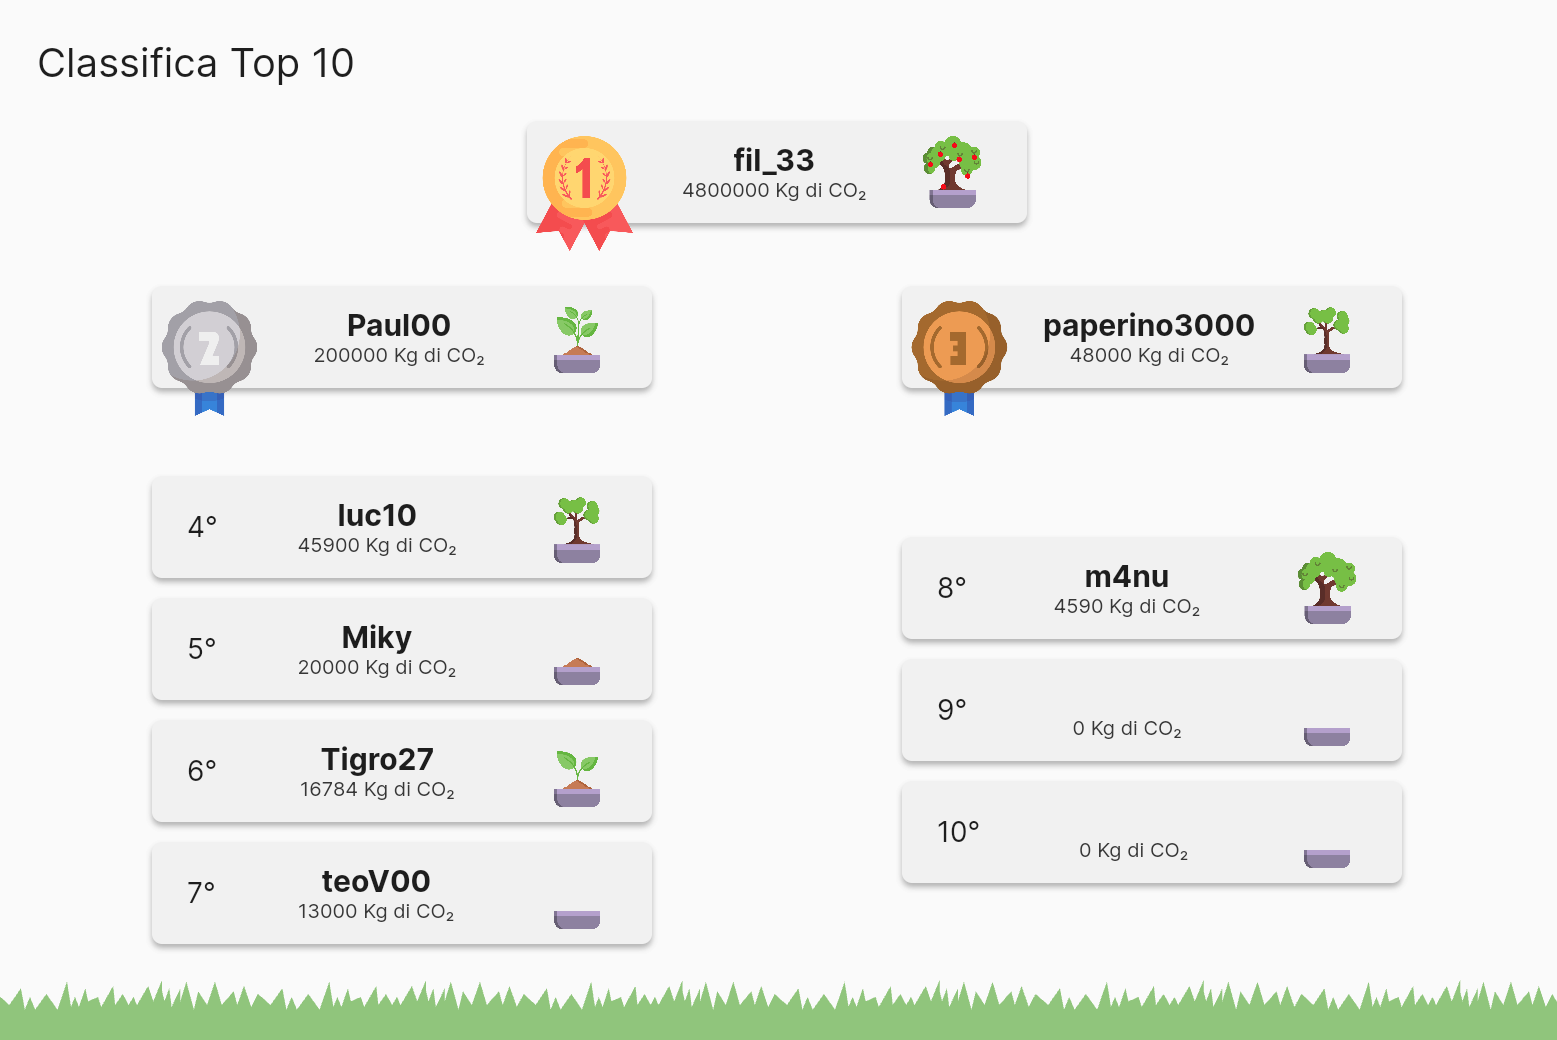
\includegraphics[width=\textwidth]{img/totem/screenshot/top10screen.png}
  \caption{Pagina della classifica conclusa.}
  \label{fig:top10screen}
\end{figure}

%
%
\subsection{Pagina Informazioni}
La pagina delle informazioni nel corso del suo concepimento ha subito vari cambiamenti, come anche precisato nel capitolo \ref{subsec:totem}, che comprendono un cambio drastico di layout passando da una semplice pagina scorrevole ad una visualizzazione a griglia contente tante \textit{tile}s (blocchi o piastrelle); la decisione d'implementare quest'ultimo è stata molto condizionata dall'esito di un sondaggio svolto su un piccolo gruppo di utenti target, che provando entrambi i mockup su device touchscreen, hanno dimostrato una maggiore preferenza per la visualizzazione a griglia in quanto più immediata, ordinata e di facile comprensione, prediligendo il tipo d'interazione \enquote*{con il tocco} (\textit{tap gesture}) per la fruizione delle informazioni al posto dello scorrimento verticale (\textit{vertical scrolling gesture}). In figura \ref{fig:infoPage} viene mostrata la pagina delle informazioni e nell \ref{fig:infoPagePopup} una delle piastrelle espanse che mostra informazioni dettagliate.

\begin{figure}
  \centering
  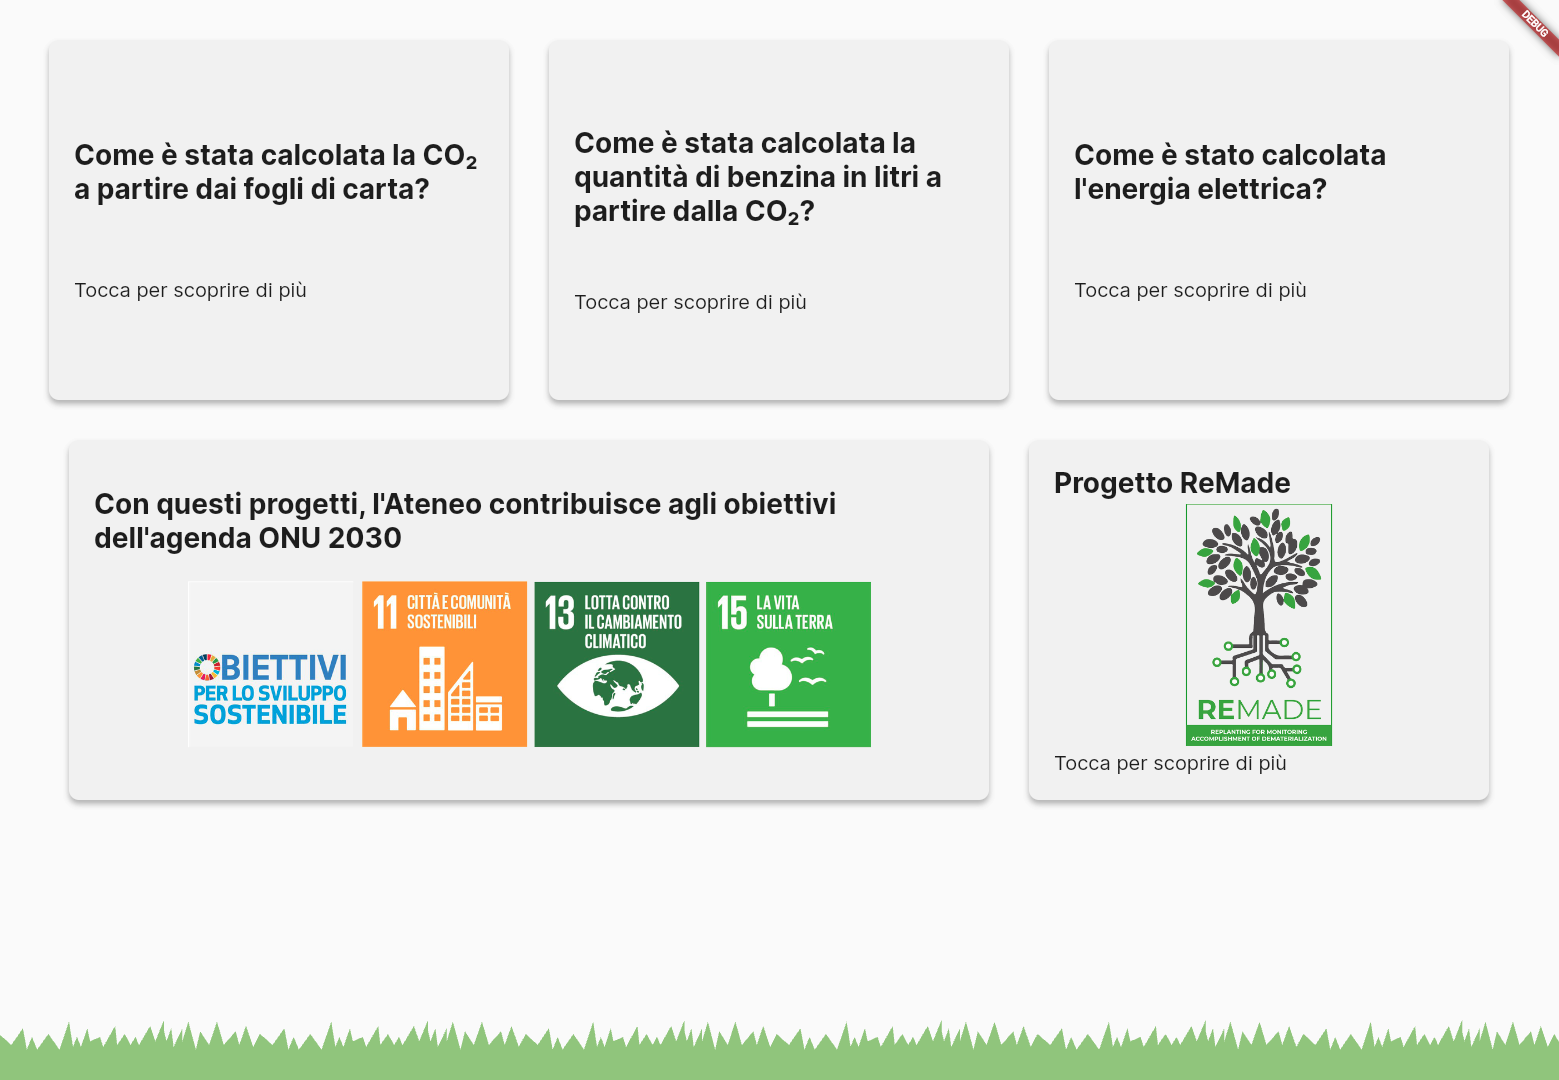
\includegraphics[width=\textwidth]{img/totem/screenshot/infoPageScreen.png}
  \caption{Pagina delle informazioni effettiva}
  \label{fig:infoPage}
\end{figure}
\begin{figure}
  \centering
  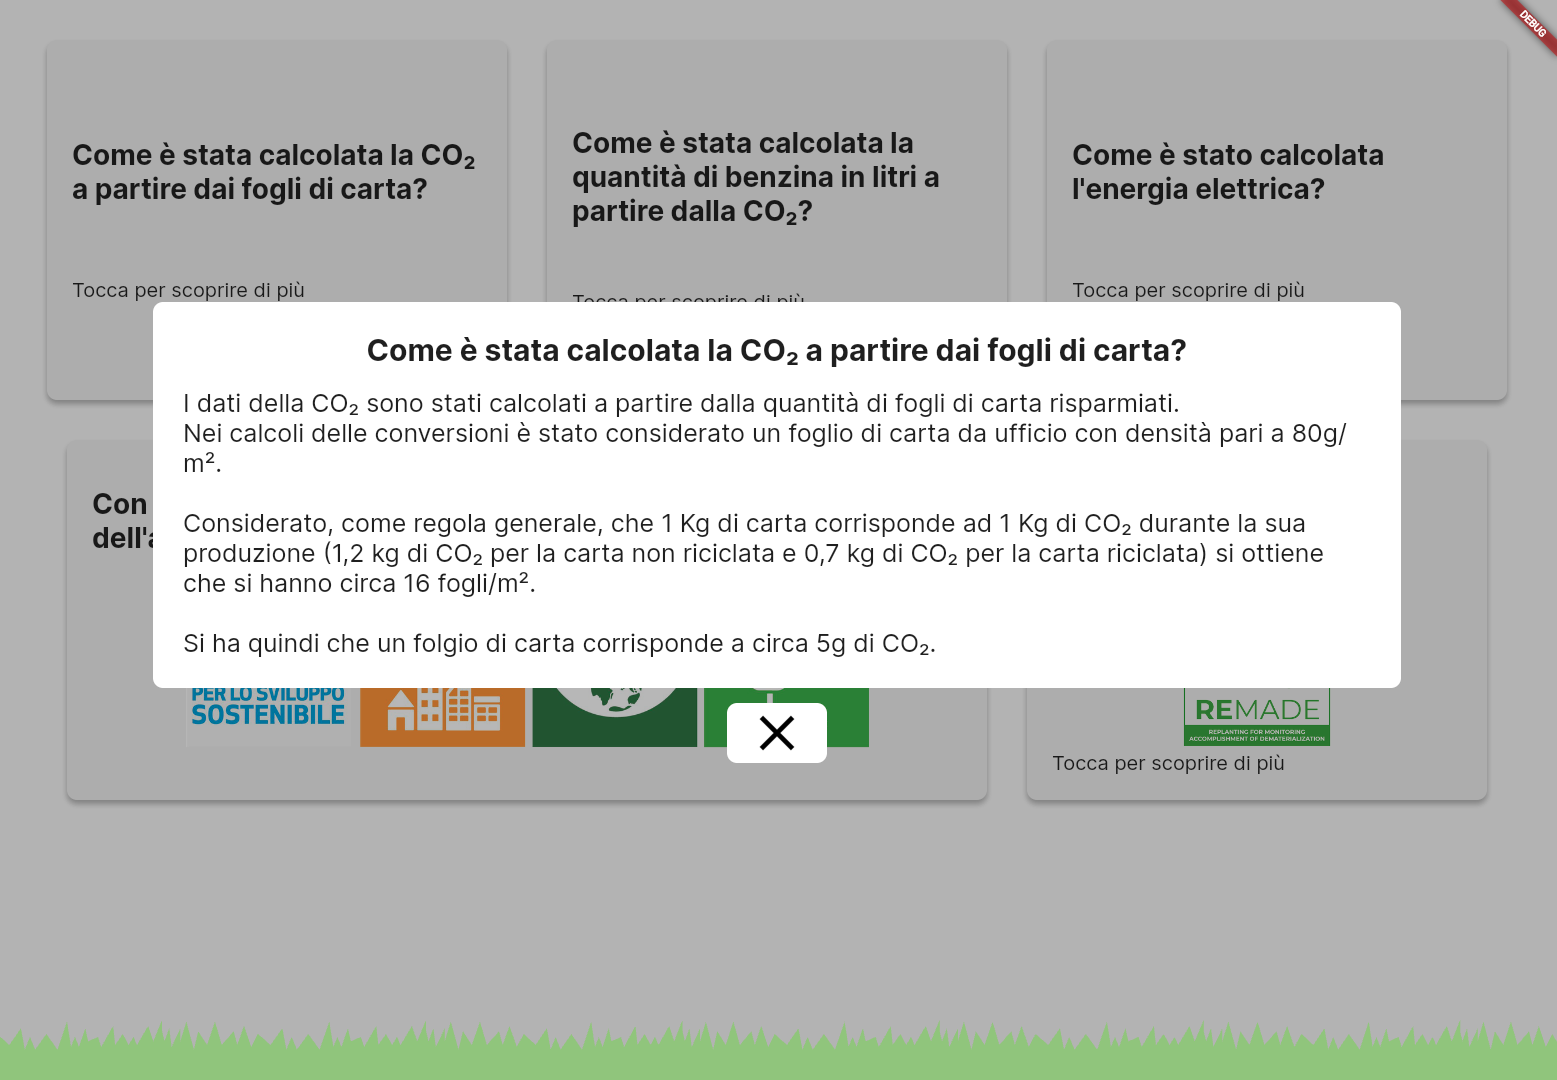
\includegraphics[width=\textwidth]{img/totem/screenshot/infoPagePopupScreen.png}
  \caption{Pagina delle informazioni: tile selezionata espansa che mostra maggiori dettagli.}
  \label{fig:infoPagePopup}
\end{figure}

Per la disposizione a griglia degli elementi è stato utilizzato il widget \texttt{GridView} utilizzando un layout personalizzato definito dalla classe \texttt{SliverQuiltedGridDelegate} del package flutter \texttt{flutter\_staggered\_grid\_view} \cite{staggeredGridView} che permette agli elementi della griglia di occupare più righe e colonne.
Attualmente sono visualizzati cinque elementi di cui uno largo il doppio (figura \ref{fig:infopageLayout}) ma è possibile aggiungerne altri, di qualsiasi dimensione compatibile alla griglia, abilitando così la navigazione verticale tramite scorrimento.

\begin{figure}
  \centering
  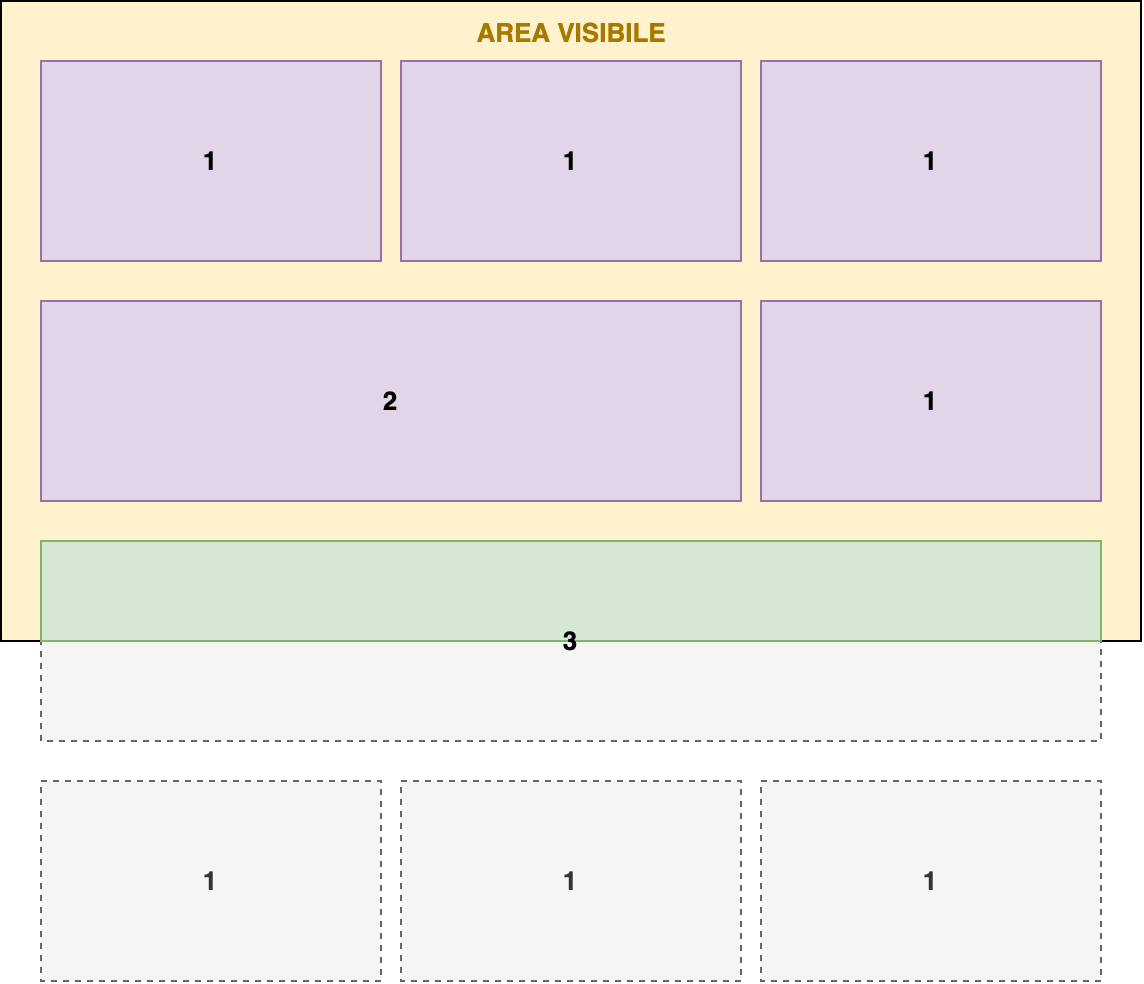
\includegraphics[width=9cm]{img/totem/layout_gridview.png}
  \caption[Layout pagina informazioni]{Layout pagina informazioni: in giallo l'area visibile, in viola le tile attualmente presenti infine in grigio quelle che potrebbero essere aggiunte, non esclusivamente in quella disposizione. I numeri presenti indicano quante colonne occupa ciascuna piastrella.}
  \label{fig:infopageLayout}
\end{figure}

\begin{lstlisting}[style=FlutterStyle, caption={}, label={lst:infoPageCode}]
  Stack(
    children: [
      Padding(
        padding: const EdgeInsets.all(50.0),
        // creazione vista a griglia
        child: GridView.custom(
          gridDelegate: SliverQuiltedGridDelegate(
            crossAxisCount: 3,
            mainAxisSpacing: 30,
            crossAxisSpacing: 30,
            repeatPattern: QuiltedGridRepeatPattern.inverted,
            pattern: const [
              // 1 riga ed 1 colonna occupata
              QuiltedGridTile(1, 1),  
              QuiltedGridTile(1, 1),
              QuiltedGridTile(1, 1),
              // 1 riga e 2 colonne occupate
              QuiltedGridTile(1, 2),
              QuiltedGridTile(1, 1),
            ],
          ),
          childrenDelegate: SliverChildBuilderDelegate(
            childCount: infoTiles.length,
            (context, index) => GestureDetector(
              child: Padding(
                padding: const EdgeInsets.only(bottom: 60.0),
                child: infoTiles[index],
              ),
              onTap: () {
                setState(() {
                  detailsWidget = infoTiles[index].getDetailsWidget();
                });
              },
            ),
          ),
        ),
      ),
      if (detailsWidget != null) ...[
        // pannello che mostra i dettagli relativi alla tile cliccata
      ],
    ],
  );
\end{lstlisting}

\section{Testing e Debug}
